% -----------------------
% preamble
% -----------------------
% Don't change preamble code yourself. If you add something(usepackage, newtheorem, newcommand, renewcommand),
% please tell them editor of institutional paper of RUMS.

%documentclass
%------------------------
\documentclass[11pt, a4paper, dvipdfmx]{jsarticle}


%usepackage
%------------------------
\usepackage{amsmath}
\usepackage{amsthm}
\usepackage[psamsfonts]{amssymb}
\usepackage{color}
\usepackage{ascmac}
\usepackage{amsfonts}
\usepackage{mathrsfs}
\usepackage{amssymb}
\usepackage{graphicx}
\usepackage{fancybox}
\usepackage{enumerate}
\usepackage{verbatim}
\usepackage{subfigure}
\usepackage{proof}
\usepackage{listings}
\usepackage{otf}
\usepackage{algorithm}
\usepackage{algorithmic}
\usepackage{tikz}
%\usepackage[dvipdfmx]{hyperref}
\usepackage[all]{xy}
\usepackage{amscd}
\usetikzlibrary{cd}

%theoremstyle
%--------------------------
\theoremstyle{definition}


%newtheoem
%--------------------------
%If you want to use theorem environment in Japanece, You can use these code. 
%Attention
%--------------------------
%all theorem enivironment number depend on only section number.
\newtheorem{Axiom}{公理}[section]
\newtheorem{Definition}[Axiom]{定義}
\newtheorem{Theorem}[Axiom]{定理}
\newtheorem{Proposition}[Axiom]{命題}
\newtheorem{Lemma}[Axiom]{補題}
\newtheorem{Corollary}[Axiom]{系}
\newtheorem{Example}[Axiom]{例}
\newtheorem{Claim}[Axiom]{主張}
\newtheorem{Property}[Axiom]{性質}
\newtheorem{Attention}[Axiom]{注意}
\newtheorem{Question}[Axiom]{問}
\newtheorem{Problem}[Axiom]{問題}
\newtheorem{Consideration}[Axiom]{考察}
\newtheorem{Alert}[Axiom]{警告}


%----------------------------
%If you want to use theorem environment with no number in Japanese, You can use these code.
\newtheorem*{Axiom*}{公理}
\newtheorem*{Definition*}{定義}
\newtheorem*{Theorem*}{定理}
\newtheorem*{Proposition*}{命題}
\newtheorem*{Lemma*}{補題}
\newtheorem*{Example*}{例}
\newtheorem*{Corollary*}{系}
\newtheorem*{Claim*}{主張}
\newtheorem*{Property*}{性質}
\newtheorem*{Attention*}{注意}
\newtheorem*{Question*}{問}
\newtheorem*{Problem*}{問題}
\newtheorem*{Consideration*}{考察}
\newtheorem*{Alert*}{警告}

%--------------------------
%If you want to use theorem environment in English, You can use these code.
%--------------------------
%all theorem enivironment number depend on only section number.
\newtheorem{Axiom+}{Axiom}[section]
\newtheorem{Definition+}[Axiom+]{Definition}
\newtheorem{Theorem+}[Axiom+]{Theorem}
\newtheorem{Proposition+}[Axiom+]{Proposition}
\newtheorem{Lemma+}[Axiom+]{Lemma}
\newtheorem{Example+}[Axiom+]{Example}
\newtheorem{Corollary+}[Axiom+]{Corollary}
\newtheorem{Claim+}[Axiom+]{Claim}
\newtheorem{Property+}[Axiom+]{Property}
\newtheorem{Attention+}[Axiom+]{Attention}
\newtheorem{Question+}[Axiom+]{Question}
\newtheorem{Problem+}[Axiom+]{Problem}
\newtheorem{Consideration+}[Axiom+]{Consideration}
\newtheorem{Alert+}{Alert}
\newtheorem{Remark+}[Axiom+]{Remark}
%commmand
%----------------------------
\newcommand{\N}{\mathbb{N}}
\newcommand{\Z}{\mathbb{Z}}
\newcommand{\Q}{\mathbb{Q}}
\newcommand{\R}{\mathbb{R}}
\newcommand{\C}{\mathbb{C}}
\newcommand{\F}{\mathcal{F}}
\newcommand{\X}{\mathcal{X}}
\newcommand{\Y}{\mathcal{Y}}
\newcommand{\Hil}{\mathcal{H}}
\newcommand{\RKHS}{\Hil_{k}}
\newcommand{\Loss}{\mathcal{L}_{D}}
\newcommand{\MLsp}{(\X, \Y, D, \Hil, \Loss)}
\newcommand{\p}{\partial}
\newcommand{\h}{\mathscr}
\newcommand{\mcal}{\mathcal}
\newcommand{\lan}{\langle}
\newcommand{\ran}{\rangle}
\newcommand{\pal}{\parallel}
\newcommand{\dip}{\displaystyle}
\newcommand{\e}{\varepsilon}
\newcommand{\dl}{\delta}
\newcommand{\pphi}{\varphi}
\newcommand{\ti}{\tilde}

\newcommand{\argmax}{\mathop{\rm arg~max}\limits}
\newcommand{\argmin}{\mathop{\rm arg~min}\limits}

\renewcommand{\P}{\mathbb{P}}
\newcommand{\Probsp}{(\Omega, \F, \P)}

%new definition macro
%-------------------------
\def\inner<#1>{\langle #1 \rangle}
%----------------------------
%documenet 
%----------------------------
% Your main code must be written between begin document and end document.
\title{Generative Adversarial Networks}
\author{小泉 孝弥}
\date{}
\begin{document}
\maketitle
%\tableofcontents
\section{Intoroduction}
近年, 機械学習
\section{Fundermetal concepts of Machine Learning}
この節では機械学習の数学的な定式化を行う. $\X$と$\Y$を有限次元線型空間とし, $\Probsp$を
完備な確率空間とする.
\begin{Definition+}(仮説空間, 仮説)\\
    $\X$から$\Y$へのなんらかの条件を満たす写像の集まりのことを仮説空間
    といい$\Hil$と表記する. すなわち,
    \begin{align*}
        \Hil = \{f:\X\to\Y~| f\text{ が満たす条件}\}
    \end{align*}
    である. (条件の具体例は後に述べる). 仮設空間$\Hil$の元のことを仮説(またはモデル)と呼ぶ.
    また, この時の$\X$を入力空間, $\Y$を出力空間と呼ぶ. 
\end{Definition+}
これ以降, 入力空間を$\R^{d}$出力空間を$\R^{m}$とする.
\begin{Definition+}(データ)\\
    $\X$と$\Y$の直積集合$\X\times\Y$の有限部分集合のことを教師ありデータという.
    また, $\X$の有限部分集合のことを教師なしデータと呼ぶ. 
\end{Definition+}
\begin{Definition+}(予測損失)\\
    $\Hil$を仮説空間とし, $(X, Y)$をデータの分布$\mathbb{P}_{\X\times\Y}$に従う確率変数と
    する. 以下で定義される$\ell:\Hil\to\R$を予測損失と呼ぶ.
    \begin{align*}
        \ell(f) = \mathbb{E}[\|f(X) - Y\|].
    \end{align*}
\end{Definition+}
予測損失が最小となるような$f\in\Hil$を求めることが機械学習の目標である. しかし, 一般にデータの分布は未知であるため
この式を解くことができない. そこで、損失関数というものを定義し、それを最適化することを考える.
\begin{Definition+}(損失関数)\\
    $\Hil$を仮説空間とする. $\Hil$から$\R$への写像$\Loss:\Hil\to\R$を損失関数(Loss function)と呼ぶ.
\end{Definition+}
\begin{Definition+}(機械学習空間)\\
    $D$をデータ, $\Hil$を仮説空間, $\Loss$を損失関数とする. 
    この時5つ組$\MLsp$を機械学習空間(Machine Learning space)という.
\end{Definition+}
\begin{Definition+}(学習, 最適仮説)\\
    $\Hil$を仮設空間, $\Loss:\Hil\to\R$を損失関数とする. 損失関数が最大または, 最小となるような
    $f^*\in\Hil$を求めること\footnote{機械学習においては厳密に損失関数が最大・最小となる関数が学習されるとは限らないが, そのような関数を求めることも学習の定義に含めるものとする. }を学習といい, $f^*\in\Hil$を最適仮説と呼ぶ.
\end{Definition+}
\begin{Definition+}(機械学習)\\
    機械学習空間$\MLsp$上での学習を機械学習という. 特に, $D$が教師ありデータの時, 教師あり機械学習と呼び, 
    教師なしデータの時, 教師なし機械学習と呼ぶ.
\end{Definition+}
\begin{Remark+}(訓練データとテストデータ)\\
    機械学習で学習を行う際は, データ$D$を全て使って学習させるのではなく, 
    データを訓練データ$D_{\text{Train}}$とテストデータ$D_{\text{Test}}$に分ける. 
    訓練データはモデルの学習に用いて, テストデータはモデルの制度の確認のために用いる. 
\end{Remark+}
\section{教師あり機械学習の具体例}
前節では, 機械学習の抽象的な枠組みを紹介したが, この説では機械学習空間の具体例を述べる.
$D = \{(x_i, y_i)\}_{i = 1}^{N}\subset\X\times\Y$を教師ありデータとする.

\subsection{単回帰分析・重回帰分析}
最初に機械学習の最も基本的なモデルである単回帰分析を紹介する. その後
その多変数拡張である重回帰分析を紹介する.
\begin{Example+}(単回帰分析)\\
    機械学習空間$\MLsp$を以下のように定義する.\\
    $\X = \R$, $\Y = \R$, 
    \begin{align*}
        \Hil &= \{f:\X\to\Y~|f(x) = wx, w\in\R\},\\
        \Loss(f) &= \sum_{i = 1}^{N}|f(x_i) - y_i|^2.
    \end{align*}
    この機械学習空間$\MLsp$上で,
    \begin{align*}
        \argmin_{f\in\Hil}\Loss(f)
    \end{align*}
    を求める問題を単回帰分析という. 単回帰分析の最適仮説$f^{*}\in\Hil$は
    \begin{align*}
        f^{*}(w) = \frac{\sum_{i = 1}^{N}x_{i}y_{i}}{\sum_{i = 1}^{N}x_{i}^2}w
    \end{align*}
    となる. また, $\Hil\simeq\R$である.
\end{Example+}
\begin{Example+}(重回帰分析)\\
    機械学習空間$\MLsp$を以下のように定義する.\\
    $\X = \R^d(N\geq d)$, $\Y = \R$, 
    \begin{align*}
        \Hil &= \{f:\X\to\Y~| f(x) = W^{T}x + b, W\in\R^{d}, b\in\R\},\\
        \Loss(f) &= \sum_{i = 1}^{N}|f(x_i) - y_i|^2.
    \end{align*}
    この機械学習空間$\MLsp$上で
    \begin{align*}
        \argmin_{f\in\Hil}\Loss(f)
    \end{align*}
    を求める問題を重回帰分析という. $X\in\R^{N\times(d + 1)}$を
    \begin{align*}
        X = \begin{pmatrix}
            1 & x_{11} & x_{12} & \cdots & x_{1d}\\
            1 & x_{21} & x_{22} & \cdots & x_{2d}\\
            \vdots & \vdots & \vdots & \ddots & \vdots\\
            1 & x_{N1} & x_{N2} & \cdots & x_{Nd}
        \end{pmatrix}
    \end{align*}
    と定義し, $\mathbf{y} = (y_{1}, y_{2}, \cdots, y_{N})^{T}\in\R^{N}$とする. この時, $\mathbf{rank}(X) = d + 1$ならば, 
    最適仮説$f^*\in\Hil$は$[b~W] = (X^TX)^{-1}X^T\mathbf{y}$とすれば
    \begin{align*}
        f^{*}(x) = [b~W]^{T}x
    \end{align*}
    である.
\end{Example+}
\subsection{線形回帰}
前小節で定義した重回帰分析は線形的なデータにしか適応できなかった. それを
基底関数と呼ばれる関数列を定義する事で, 非線形データにも対応することができる.
\begin{Definition+}(基底関数)\\
    $\X$を入力空間とし, 任意に$d\in\N$をとる. $\X$上の連続関数列$\{\phi_{n}\}_{n = 1}^{d}\subset C(\X, \X)$
    が一次独立であるとき, $\Phi = (\phi_1, \phi_2, \cdots, \phi_d)^{T}:\X\to\X^{d}$を基底関数(basis function)と呼ぶ.
\end{Definition+}
\begin{Example+}(多項式回帰)\\
    機械学習空間$\MLsp$を以下のように定義する.\\
    $\X = \R, \Y = \R$, 
    \begin{align*}
        \Hil &= \{f:\X\to\Y~| f(x) = W^{T}\Phi(x), W\in\R^{d + 1}\},\\
        \Loss(f) &= \sum_{i = 1}^{N}|f(x_i) - y_i|^2.
    \end{align*}
    ここで, $\phi_{n}(x) = x^{n}$, $n\in\{0, 1, \cdots, d\}$とする.\\
    この機械学習空間$\MLsp$上で
    \begin{align*}
        \argmin_{f\in\Hil}\Loss(f)
    \end{align*}
    を求める問題を多項式回帰という. $X = [\phi_{1}(x_1), \phi_{2}(x_{2}), \cdots, \phi_{N}(x_N)]^{T}\in\R^{N\times d}$とし, 
    $\mathbf{y} = (y_{1}, y_{2}, \cdots, y_{N})^{T}\in\R^{N}$とする. この時, 最適仮説$f^{*}$は
    重回帰分析と同様に$W = (X^TX)^{-1}X^T\mathbf{y}$とすれば
    \begin{align*}
        f^{*}(x) = W^{T}x
    \end{align*}
    である. 
\end{Example+}
\begin{Remark+}(ハイパーパラメータと学習パラメータ)\\
    多項式回帰の多項式の次数$d\in$や基底関数$\{\phi_{n}\}_{n = 1}^{d}$のように
    コンピュータに学習させるのではなく, 機械学習モデルの設計者が設定するパラメータのことを
    ハイパーパラメータと呼ぶ. 一方, $W\in\R^{d + 1}$のように, データからコンピュータが自動で学習
    するパラメータのことを学習パラメータと呼ぶ.
\end{Remark+}
\subsection{過学習と正則化}
前節の多項式回帰で学習を行うと以下のグラフのように, 訓練データに過剰適合してしまい, 未知のデータに関しての汎化性能
が小さくなってしまうことを過学習(overfitting)という. 
\begin{figure}[H]
    \centering
    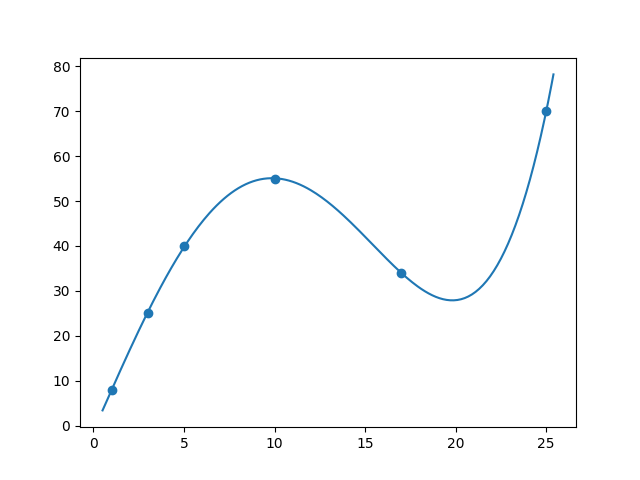
\includegraphics[width = 9.0cm]{overfitting_PR.png}
    \caption{$d = 4$の時の多項式回帰の過学習}
\end{figure}
過学習を防ぐための手法が正則化である.
\begin{Definition+}(正則化)\\
    $\Loss:\Hil\to\R$を損失関数とする. $\Loss^{R} := \Loss + L^{R}$とする.
    この時, $\Loss^{R}$を$\Loss$の正則化と呼び, $L^R$を正則化項と呼ぶ.
\end{Definition+}
\begin{Example+}(Lasso正則化多項式回帰)\\
    $\lambda\in\R^{+}$, $d\in\N$を任意にとる.機械学習空間$\MLsp$を以下のように定義する.\\
    $\X = \R, \Y = \R$, 
    \begin{align*}
        \Hil &= \{f:\X\to\Y~| f(x) = W^{T}\Phi(x), W\in\R^{d + 1}\},\\
        \Loss(f) &= \sum_{i = 1}^{N}|f(x_i) - y_i|^2+\lambda W^TW.\hspace{10pt} (W\text{は$f$のパラメータ})
    \end{align*}
    ここで, $\phi_{n}(x) = x^{n}$, $n\in\{0, 1, \cdots, d\}$とする.\\
    この機械学習空間$\MLsp$上で
    \begin{align*}
        \argmin_{f\in\Hil}\Loss(f)
    \end{align*}
    を求める問題をLasso正則化多項式回帰という. 通常の多項式回帰の時と同様に, $X = [\phi_{1}(x_1), \phi_{2}(x_{2}), \cdots, \phi_{N}(x_N)]^{T}\in\R^{N\times d}$とし, 
    $\mathbf{y} = (y_{1}, y_{2}, \cdots, y_{N})^{T}\in\R^{N}$とする. この時, 最適仮説$f^{*}$は
    $W = (X^TX + \lambda I)^{-1}X^T\mathbf{y}$とすれば
    \begin{align*}
        f^{*}(x) = W^{T}x
    \end{align*}
    である. 
\end{Example+}
正則化の結果が以下のグラフである.
\begin{figure}[H]
    \centering
    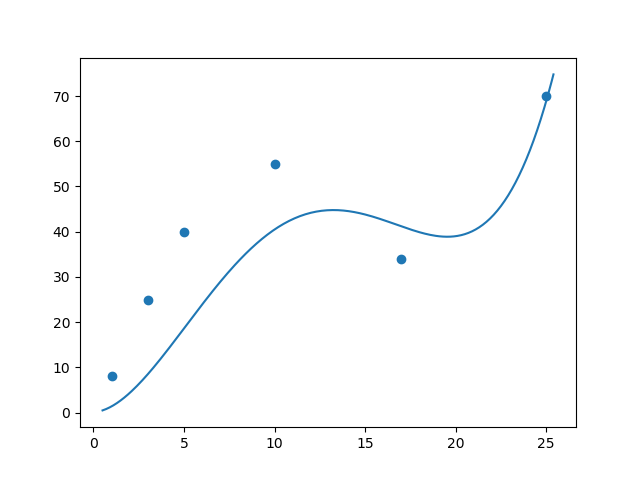
\includegraphics[width = 7.5cm]{regulaer_PR.png}
    \caption{$\lambda = 700$, $d = 4$の時のLasso正則化多項式回帰}
\end{figure}
このように正則化をすることで, パラメータが大きくなりすぎることを防ぐことで過学習を防ぐことができる.
\begin{Remark+}(未学習について)\\
    正則化を行う際にパラメータ$\lambda\in\R^+$\footnote{正則化パラメータという.}は自分で
    決める必要がある. その際に$\lambda$の値を大きくしすぎると未学習(underfitting)という問題が発生する.
    未学習とは訓練データに対してモデルが十分に適合できていないことである.
    \begin{figure}[H]
        \centering
        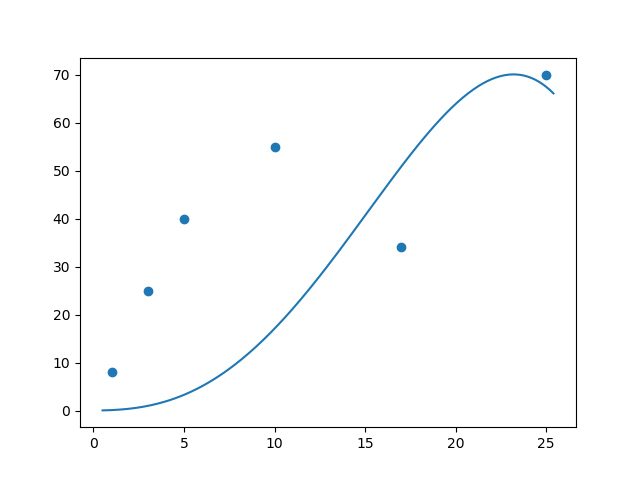
\includegraphics[width=7.5cm]{underfitting_PR.png}
        \caption{$\alpha = 30000$, $d = 4$の時のLasso正則化多項式回帰の未学習}
    \end{figure}
    このように, 正則化パラメータは適切に選ぶことが大切である. 
\end{Remark+}
\subsection{ロジスティック回帰と勾配降下法}
最後の具体例として, ロジスティック回帰を紹介する. 
ロジスティック回帰は分類問題を解くための手法の1つである. 
\begin{Example+}(ロジスティック回帰)\\
    機械学習空間$\MLsp$を以下のように定義する.\\
    $\X=\R^d$, $\Y = \R^m$, 
    \begin{align*}
        \Hil &= \{f:\X\to\Y | f(x) = \sigma(W^{\top}x), W\in\R^d\},\\
        \Loss(f) &= \sum_{i = 1}^{N}(-y_{i}\log f(x_{i}) - (1 - y_{i})\log(1 - f(x))).
    \end{align*}
\end{Example+}
\section{Deep Learning}
\subsection{Neural Network}
\subsection{The Universal Theorem of Neural Network}
\section{Generative Adversarial Networks}
\subsection{GANの定式化}
$\Probsp$を完備な確率空間とする.  
$\X$, $\Y$を線型空間とする. 
\begin{align*}
    \Hil_1 &= \{G:\mathcal{Z}\to\X~| G\text{はニューラルネット}\},\\
    \Hil_{2} &= \{D:\X\to [0, 1]~| D\text{はニューラルネット}\}
\end{align*}
ここで、$\mathcal{Z}$は潜在空間と呼ばれる$\R^{\dim\X}$の線型部分空間である.
また, 確率変数$Z:\Omega\to\mathcal{Z}$に対し, $g(Z)$が従う確率分布を$\mathbb{P}_{}$
\section{Applications of GANs}

\begin{thebibliography}{20}
    \bibitem{GAN} Ian J. Goodfellow, Jean Pouget-Abadie, Mehdi Mirza, Bing Xu, David Warde-Farley, Sherjil Ozair, Aaron Courville and Yoshua Bengio. 
    Generative adversarial nets. In Advances in Neural Information Processing Systems, 2014.
    \bibitem{SGAN}Takeru Miyato, Toshiki Kataoka, Masanori Koyama and Yuichi Yoshida, Spectral Normalization for Generative Adversarial Networks, 
    International Conference on Learning Representations, 2018.
\end{thebibliography}

\end{document}